\documentclass[12pt,a4paper]{article}
% \usepackage[english]{babel}
% \usepackage[utf8x]{inputenc}

\usepackage{graphicx} % Required for inserting images.
\usepackage[margin=25mm]{geometry}
\parskip 4.2pt  % Sets spacing between paragraphs.
% \renewcommand{\baselinestretch}{1.5}  % Uncomment for 1.5 spacing between lines.
\parindent 8.4pt  % Sets leading space for paragraphs.
\usepackage[font=sf]{caption} % Changes font of captions.

\usepackage{amsmath}
\usepackage{amsfonts}
\usepackage{amssymb}
\usepackage{siunitx}
\usepackage{verbatim}
\usepackage{hyperref} % Required for inserting clickable links.
\usepackage{natbib} % Required for APA-style citations.


\title{Heist at the Royal Castle}
\author{Saif Nazir and Hania Kashif}

\begin{document}
\maketitle

% \begin{abstract}
% \end{abstract}

\section{Introduction and Synopsis}\label{sec:intro}
Our project proposal introduces Heist at the Royal Castle, a 2D top-down game crafted using C++ and the SDL library, employing object-oriented programming for its development. In this game, the player assumes the role of a thief on a daring mission.

The primary goal is to infiltrate a castle, find the three keys to unlock the treasure, find where the treasure is hidden, and make it out of the castle with at least one life of 3 initial lives. The player also encounters enemies and has to overcome obstacles during the heist. 

Object-oriented programming principles drive the project, providing modularity and flexibility to the codebase. Key elements like the thief, enemies, keys, and the environment block such as rocks and trees are represented as distinct objects, allowing for easy expansion and maintenance. This project exemplifies the benefits of object-oriented programming in game development by promoting code reusability and maintainability, while also providing an interactive implementation.
\section{SDL Concepts}\label{sec:SDL concepts}
To create Heist at the Royal Castle using C++ and the SDL library, we can leverage various SDL concepts to develop the game effectively. Here's how SDL concepts can be applied to different aspects of the game:
\begin{itemize}
    \item We will use SDL to create the window and render the envionment and graphics such as the thief, lives, keys and enemies.
    \item We will also use SDL to control the character using the keyboard, output sound, and enable user interaction with the game.
    \item It can also be used to make the environment more interactive and to handle collisions and enemies.
\end{itemize}

\section{Object Oriented Design Approach}\label{sec:oop approach}
We will be using Object Oriented Design Approach to implement the game, which can be demonstrated as follows:
\begin{itemize}
\item Class-Based Structure: Implement the game's components $($e.g., thief character, enemies, keys, castle) as classes, encapsulating their properties and behaviors within these objects.
\item Inheritance: Utilize inheritance to create a hierarchy of game elements. For example, a base "Character" class can serve as the parent class for the thief and enemies, inheriting common attributes like position and movement.
\item Polymorphism: Implement polymorphism to handle interactions between different game objects. For instance, different objects (keys, enemies, treasures) may have unique interactions with the thief character.
\item Abstraction: Abstract away complex details by encapsulating behaviors and attributes within classes. This simplifies the management of game elements and allows for easier code maintenance and debugging.
\item Encapsulation: Use encapsulation to protect the internal state of objects. This ensures that the game's data remains consistent and prevents unintended access or modification of critical variables.
\item Modularity: Promote code modularity by dividing the game into self-contained objects. This approach allows for easier development, testing, and reusability of game elements.
\item Game State Management: Create a game state manager to switch between various game states, such as level selection, gameplay, and endgame scenarios. Each state can be represented as a separate class.
\item Code Reusability: Leverage OOP to promote code reusability. Reusable classes can be employed in different game scenarios, saving development time and ensuring consistent functionality.
\end{itemize}
We will also be making use of good coding practices as mentioned in the provided document.

\section{Gameplay Instructions}\label{sec:game instructions}

The game has the main character as the thief, and the objective is to break into a castle, steal the treasure and make it out with at least one life. The gameplay instructions can be given as:
\begin{itemize}
    \item Arrow keys contorl the character movement and only the pathways can be traversed by the thief. Some places cannot be accessed, like the thief cannot go over trees, and might lose a life if the player drowns in a lake for example.
    \item The map of the castle has enemies that are patrolling various pathways, and they fire at the thief if the player comes in their path. We cannot implement AI to make the enemies follow the thief, so we are just hard programming the enemies to shoot if the thief gets in their way.
    \item The game initially starts with 3 lives and if the thief is hit by the enemies or if the player traversed an area such as a lake or a bog, then one life is lost. 
    \item The player has to find 3 keys which are partially hidden in different places to be able to unlock the treasure.
    \item The treasure is also hidden in one of 2 or 3 random places, and we will implement the game in a way that the treausre is hidden randomly when the game starts.
    \item After finding the keys and getting the treasure, the thief must make it outside the castle (ie. traverse back the same way) with at least one life remaining.
    \item The player gets bonus points if a secret gem is discovered. It will be spawned in one of 3 random places and the player can finish the game without getting the gem as well.
    \item Pressing the escape key will bring the player to the game menu where options such as sound, exit, ect. will be given.
\end{itemize}
We will try to implement as much of the game logic and features as the time allows, but this structure might be subject to change and will be updated accordingly in the weekly updates.

\subsection{Game Screens}\label{sec:game screens}

A barebone design of the game is given below. We have also zipped the relevant sprites and material we will be using to make the game. If we do find some other material, we will include that for our sprites too.

\begin{figure}[htbp!]
\begin{center}
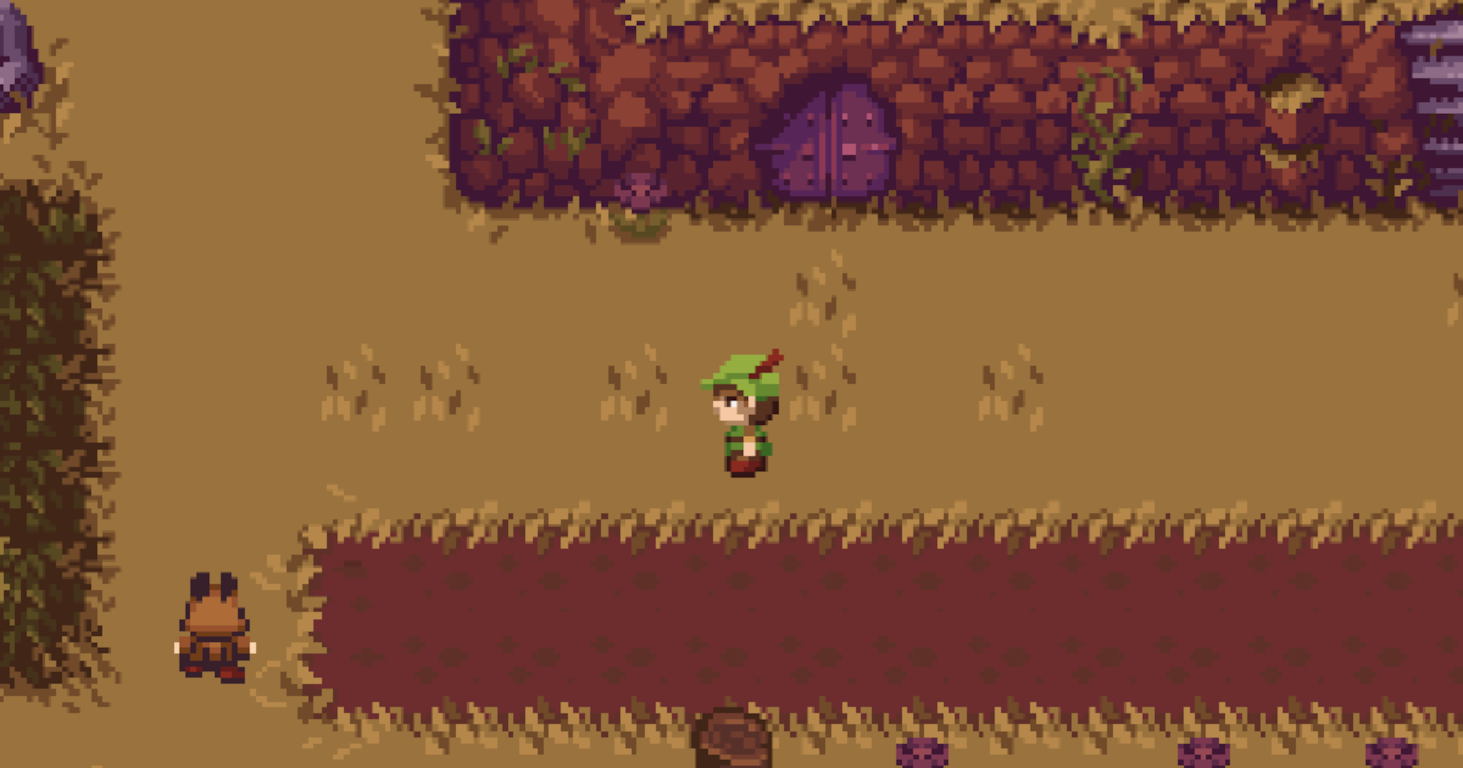
\includegraphics[width=0.5\columnwidth]{menu.png}
\end{center}
\caption{Basic menuscreen for the game. We will implement it with pixellated sprites}
\label{fig:menu}
\end{figure}

\begin{figure}[htbp!]
\begin{center}
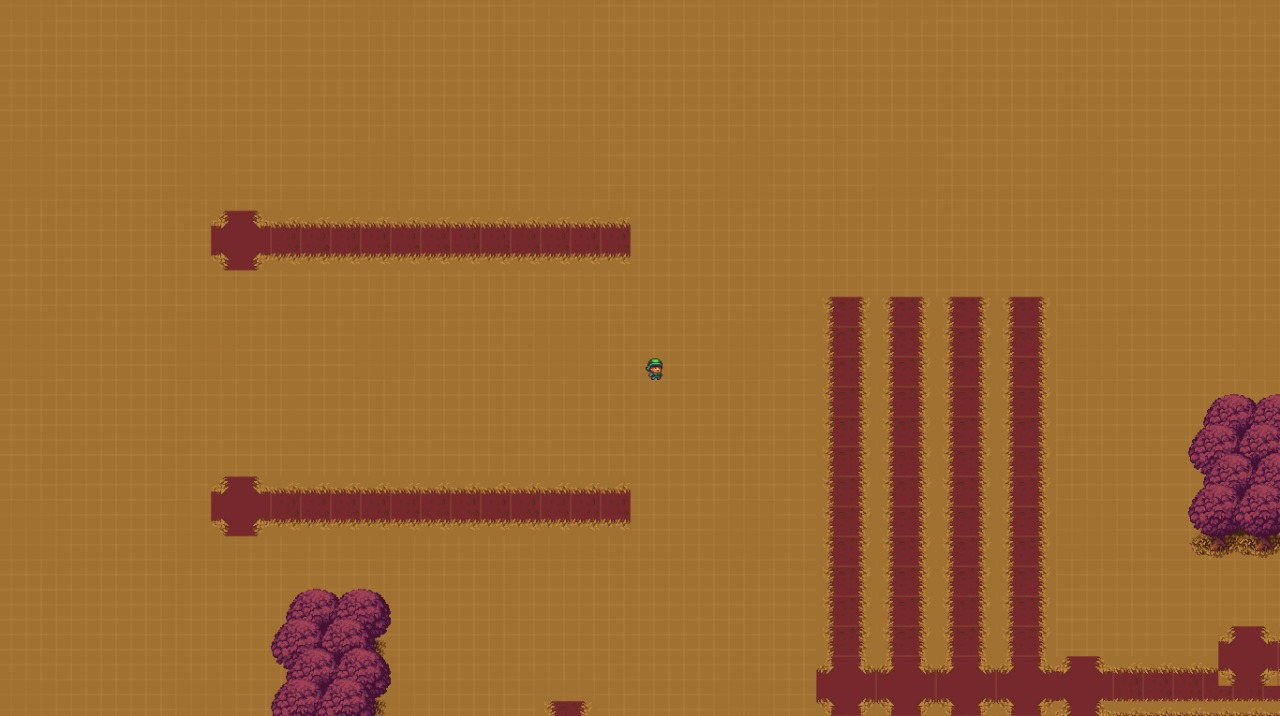
\includegraphics[width=0.5\columnwidth]{game initial stage.jpg}
\end{center}
\caption{A scene from the game in which the character is shown in the middle. The environment is not yet fully constructed, but will be worked on in the coming weeks. Methods to move the character have been implemented, and the frame also moves relative to the character.}
\label{fig:gamewon}
\end{figure}

\begin{figure}[htbp!]
\begin{center}
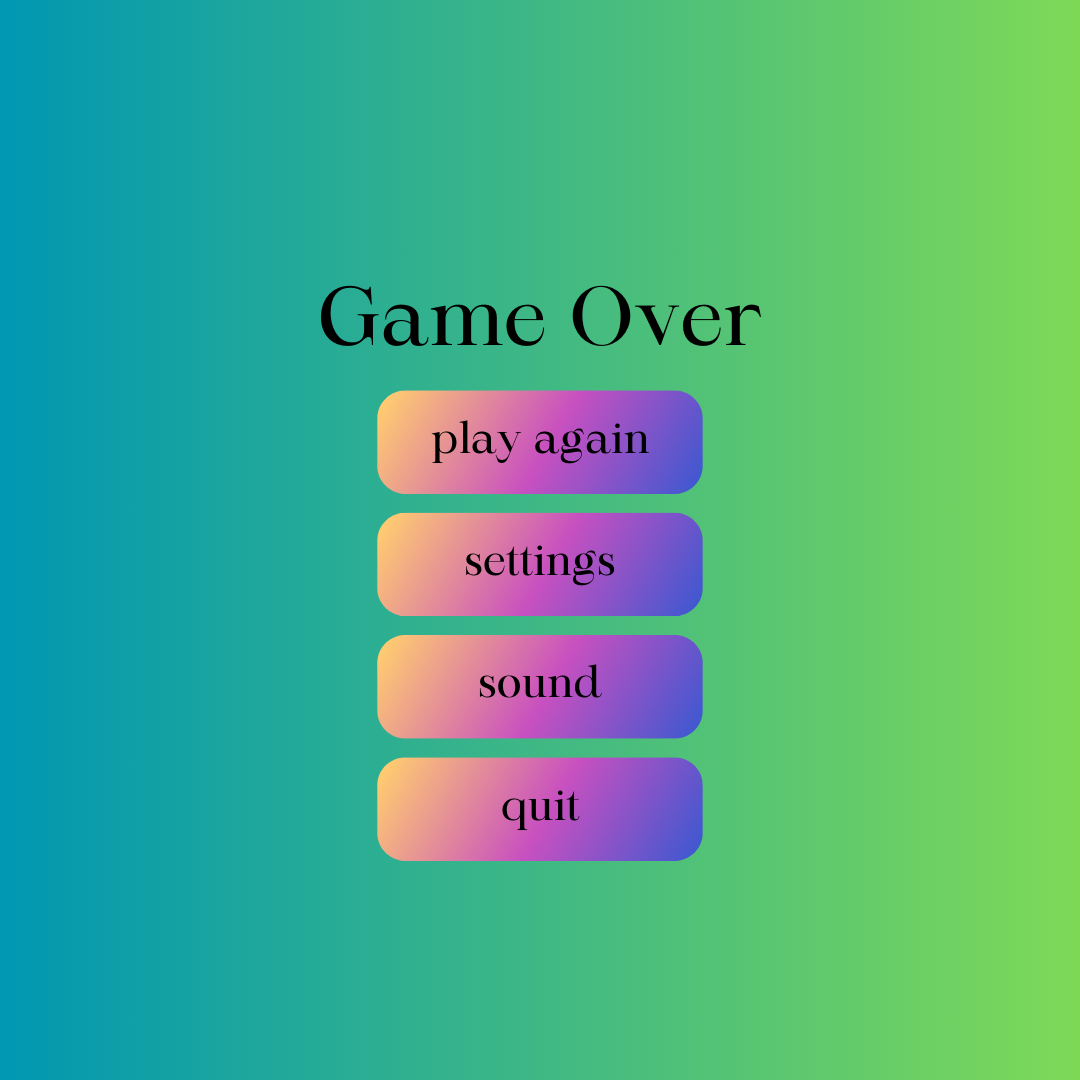
\includegraphics[width=0.5\columnwidth]{gameover.png}
\end{center}
\caption{Basic game over screen for the game. We will implement it with pixellated sprites}
\label{fig:gameover}
\end{figure}

\begin{figure}[htbp!]
\begin{center}
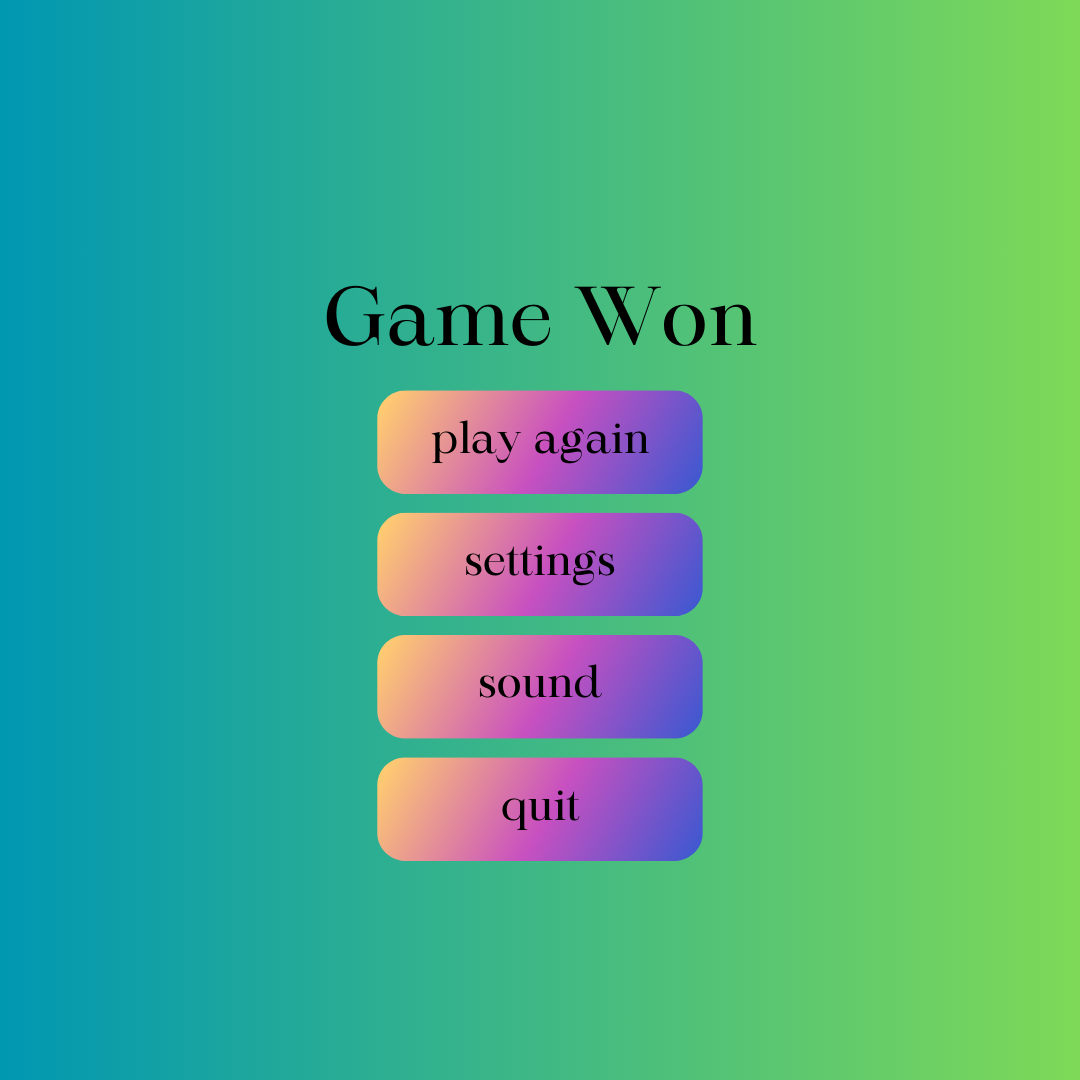
\includegraphics[width=0.5\columnwidth]{gamewon.png}
\end{center}
\caption{Basic game won screen for the game. We will implement it with pixellated sprites}
\label{fig:gamewon}
\end{figure}

\section{Project Timeline}\label{sec:Timeline}

In the first week, we were able to make some of the game screens required such as the main screen, menuscreen and game end screen, though all the functions were not wholly implemented. The game screen shows the main map and the character in between, who also moves using the arrow keys. We were also able to implement the moving frame logic, ie. the frame is dynamic when the player reaches to a specific point on the screen and the view can be shifted to show the rest of the map.

By the second week we will try to implement most of the classes and design the map completely, while adding variables for the life of the player as well. We might also try to complete the main game score logic.

By third week we are planing to get the game into functional mode by implementing most of the interactions with the character and the enemies, and also take down the random position of the treasure, the keys and the secret gem.

By fourth week, we will try to finalzise the game and add on to the remaining features if any. Note that the project timleline can be changed, and so can a few of our implementations if we feel the need to do so.

\section{Materials and References}\label{sec:References}

We will be using sprites that we have downloaded from the internet, and audios that are availible online. All the relevant material has been zipped in the submission. We might look up some more sprites and audios in the coming weeks as well.
The UML diagram was made on LUCID online, so we are linking it here as well.
\href{https://lucid.app/lucidchart/eebd1889-03d9-42c5-a1c6-9e129e79c21b/edit?viewport_loc=1611%2C-914%2C2270%2C1094%2C0_0&invitationId=inv_76e59cee-f25e-4bd6-b04e-aeb0cfabf7f4}{UML Diagram}

\end{document}